\section{Product}
Momenteel kan het prototype de locatie uit de GPS halen middels I2C communicatie
en deze middels SPI doorgeven aan de LoRa module.
Via de KPN Portal komt het binnen bij onze API, waar de binnengekomen berichten
in de database gelogd worden. Vanaf de KPN naar onze server loopt het verkeer via
een HTTPS verbinding.

De server draait op CentOS7, waarbinnen een Apache webserver en een MariaDB SQL-
server draaien om de gegevens op te slaan en te verwerken.

Verder is de server in staat om van de meetpunten een kaart te tonen op een
webpagina. Hierop zijn de meetpunten te selecteren om toe te voegen aan een perceel.

In deze ontwikkelfase wordt er nog gebruik gemaakt van het KPN LoRa netwerk, wat
natuurlijk in de doelgebieden niet beschikbaar is. Daarom zal er daar met een
eigen gateway en lokale server gewerkt moeten worden om de GPS-data van de Smart
Markers te verzamelen en verwerken.

% TODO Wat doen de markers nu precies qua locatie en hoe gaat dit in de toekomst?

Daarnaast kan de energievoorziening gerealiseerd worden, op dit moment is het
prototype alleen in gebruik geweest met een laptop. Te denken valt aan een
(interne), oplaadbare, stroomvoorziening om de marker makkelijker in het veld te
kunnen plaatsen.

Verder hebben we het met het Kadaster gehad over manieren om de percelen met
minder handwerk te maken, bijvoorbeeld door het analyseren van sattelietbeelden.

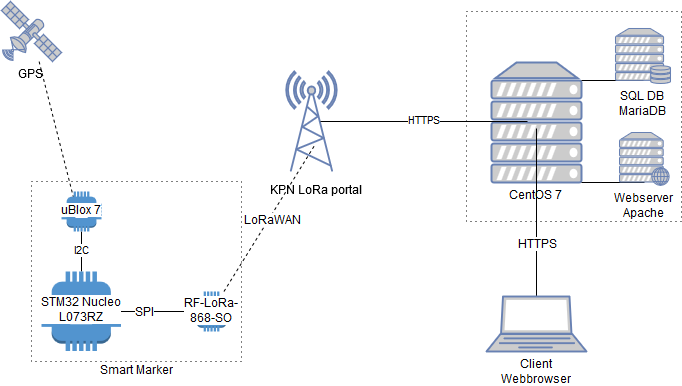
\includegraphics[width=\linewidth]{final_report/All_parts.png}
